\documentclass[answers]{exam}

\usepackage[dvipsnames]{xcolor}
\usepackage{amsmath}
\usepackage{amsfonts}
\usepackage{amsthm}
\usepackage{microtype}
\usepackage{siunitx}
\DeclareSIUnit\year{yr}
\usepackage{pgfplots}
\usepackage{graphicx}
\usepackage{sidecap}
\sidecaptionvpos{figure}{c}
\usepackage{float}
\usepackage{gensymb}
\usepackage{tkz-euclide}
\usetkzobj{all}
\usepackage{commath}

\newtheorem*{thm}{Theorem}

\renewcommand*{\thefootnote}{\fnsymbol{footnote}}

% russian integral
\usepackage{scalerel}
\DeclareMathOperator*{\rint}{\scalerel*{\rotatebox{17}{$\!\int\!$}}{\int}}

% \qformat{Question \thequestion: \thequestiontitle\hfill}

\begin{document}

\section*{NCEA Level 2 Physics\\Assignment M2: Energies}

\paragraph{Important note (please read this).} Some of these questions may appear to give less information than you think
you need. Nonetheless, they are all possible! This is illustrative of the power of energy conservation as a tool. You will
find it particularly useful, for each scenario, to begin by thinking about any forces that are acting and any energy changes
that are taking place. \emph{Diagrams are often helpful; as well as pictures of the scenario and force diagrams, you might
also want to draw rough flowcharts showing energy changes.}

Please be reminded as well that (1) the questions do not necessarily increase in difficulty as you go down the page (i.e.
the later ones might be easy), and (2) I would prefer you attempt as many problems as possible, rather than spending the
whole week stuck on one and ignoring the rest. Most of these questions are difficult, but it should be possible for you
to at least come up with some kind of plausible direction, at least.

\begin{questions}
  \question Describe as many energy changes as you can that are associated with an aeroplane during a flight,
            from the moment the doors close at one airport to the moment the doors open at the destination.
            \emph{Do not perform any calculations.}

            (Hints: every time a force acts, there is an energy change going on. Some relevant forces might
            include friction or thrust (of the engine) --- there are several more that I can think of. Draw
            a flowchart showing flow of energy from one form to another mediated by these forces.)
  \question Suppose I have a spring of (unstretched) length \SI{5.00}{\centi\metre}.
    \begin{parts}
      \item I hang my spring vertically, so the top is fixed and the bottom is free to
            move up and down; I hang a \SI{100}{\gram} mass on the bottom. The new
            length of the spring is \SI{6.50}{\centi\metre}.

            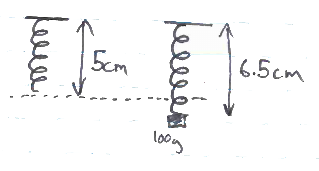
\includegraphics[width=0.3\textwidth]{2spring1}
        \begin{subparts}
          \subpart Draw a diagram showing both forces acting on the hanging mass. Given that
                   the mass is not accelerating (it is stationary), what can you say about these
                   two forces?
          \subpart Show that the spring constant of the spring is $ k = \SI{65.4}{\kilo\gram\per\second\squared} $.
        \end{subparts}
      \item Suppose now I align the \emph{same} spring horizontally, with the \emph{same} mass still attached at one end and the other end fixed.
            The mass is lying on a frictionless surface and is free to move backwards and forwards. I pull the mass a distance \SI{3.00}{\centi\metre}
            from its resting place, stretching the spring; I then let the mass go.

            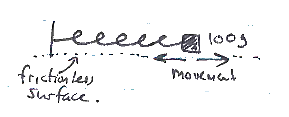
\includegraphics[width=0.3\textwidth]{2spring2}
        \begin{subparts}
          \subpart Draw a diagram showing the direction of the forces on the mass and the velocity of the mass at various points in time. (Hint: the
                   only non-balanced force acting is the elastic force, and it always acts in the opposite direction to the velocity.) In particular, note
                   on your diagram the point where the velocity of the mass is largest.
          \subpart Show that the maximum velocity of the mass is \SI{4.43}{\metre\per\second}.
        \end{subparts}
    \end{parts}
  \clearpage
  \question Petrol, as used in cars, has an energy content of roughly \SI{46.7e6}{\joule\per\liter}.\footnote{This is something that one
            would measure in chemistry: if you have done the level 2 chemistry topic on chemical reaction rates, this is the standard
            enthalpy of combustion of petrol. It can be measured by burning a set amount of petrol under a beaker containing water
            and measuring the temperature change of the water. As physicists, we just care what the number is, not the way we get it!}
    \begin{parts}
      \part A car (mass \SI{1350}{\kilo\gram}) accelerates smoothly from rest to a speed of \SI{50}{\kilo\metre\per\hour}. Assuming
            that only negligible energy is lost to friction, how many litres of petrol did the car burn? (You should obtain
            a number that is very small. One litre of petrol has a rough mass of \SI{1}{\kilo\gram}, so the amount of mass lost by
            burning the petrol is very small compared to the total mass of the car, and so we don't need to take it into account.)
      \part The car travels in a straight line for 100 kilometres, at a constant speed of \SI{50}{\kilo\metre\per\hour}
            (i.e. it does not accelerate at all); it burns \SI{5.3}{\liter} of petrol.
        \begin{subparts}
          \subpart Assuming that the only energy loss is due to friction, how much energy is converted from chemical energy
                   to heat and sound energy by the friction force? (In other words, how much work does the friction force do to the car?)
          \subpart Assuming the friction force is constant, calculate its magnitude.
          \subpart The engine cuts out suddenly. How long does it take for the car to coast to a halt?
        \end{subparts}
    \end{parts}
  \question Two toy cars are initially moving in the same direction at different speeds. One has a mass \SI{100}{\gram} and is moving
            at a speed \SI{1.0}{\metre\per\second}, the other, behind it, has a mass \SI{50}{\gram} and is moving at a speed \SI{2.0}{\metre\per\second}.
            When the faster car catches up and the two cars collide, they stick together and move as one mass.
    \begin{parts}
      \part Using conservation of momentum, show that the final speed of the clumped cars is \SI{1.3}{\metre\per\second}.
      \part Show that kinetic energy is \emph{not} conserved in this collision. How much kinetic energy is lost during the collision?
      \part Explain why we have not just disproved the law of conservation of energy. (Hint: state the law of conservation
            of energy carefully.)
    \end{parts}
\end{questions}

\vspace*{0.3\textheight}
Please turn over for some useful facts!

\clearpage
\subsection*{Useful facts}
\paragraph{Newton's laws}
\begin{enumerate}
  \item If the total force on an object is zero, then the object has no acceleration (its speed and direction of movement are constant).
  \item The acceleration felt by an object of mass $ m $ when acted upon by a force $ F $ is $ a = F/m $. Equivalently,
        if a constant force $ F $ acts for a time $ t $ on an object then the change in momentum is $ \Delta p = Ft $.
  \item If an object $ A $ exerts a force on an object $ B $, then object $ B $ exerts an equal and opposite force on object $ A $.
\end{enumerate}

\paragraph{Force laws}
\begin{itemize}
  \item Gravity: $ F = mg $, towards the centre of the earth.
  \item Elastic (Hooke's law): $ F = kx $, opposing the displacement.
\end{itemize}

Other forces: normal, friction/air resistance, electromagnetic, ...

\paragraph{Conservation laws}
\begin{itemize}
  \item In a closed system (i.e. a system where no external forces act), the total momentum is conserved.
  \item In a closed system (i.e. a system where no external forces act), the total energy is conserved.
\end{itemize}

\paragraph{Energy laws}
When a force $ F $ acts over a distance $ d $, the energy transferred is $ W = Fd $.

\begin{itemize}
  \item Gravity potential: $ \Delta E = mg \Delta x $.
  \item Elastic potential: $ \Delta E = \frac{1}{2} k x^2 $.
  \item Kinetic: $ E_K = \frac{1}{2} mv^2 $.
\end{itemize}

Other types of energy: heat, light, sound, electromagnetic, rotational kinetic, ...


\vspace*{\fill}
This version: \today

\end{document}
